\chapter{Experimentation}
\label{cha:exp2}

The current chapter will present the progress that has been achieved during the time devoted to the project. Section 4.1 will state on which experimental conditions work is being performed. Section 4.2 will present performance results of serial and parallel versions of the shallow water simulation as defined in Chapter 3.

It is worth noting that all code developed for the project, along with scripts for repeating executions, obtaining statistics and creating relevant plots, may be found in~\cite{arturo_isai_castro_perpuli_2015_16985}. Previous serial, parallel and experimental versions of the code have also been added as a reference in the same repository.

\section{Conditions of experimentation}

All experiments were conducted with 10 repetitions. A 95\% confidence level is considered in the plots of this project, in accordance with the material and experienced obtained during the COMP60611 course. The reported performance results correspond to the minimum observed time of execution over the 10 repetitions.

All C versions discussed in the results are compiled using the \texttt{-O3} optimisation flag, both on the Intel icc and the GCC compilers.

The problem sizes were chosen to allow proper vectorisation of the code in the OpenCL versions targeting the Xeon Phi processor, specifically. The work sizes must be multiples of 32 for better performance~\cite{Intel2014}. Since the code uses one extra element for padding, then the problem size must be a multiple of 32, minus one element. The actual 

\begin{table}[!ht]
\begin{center}
\centerline{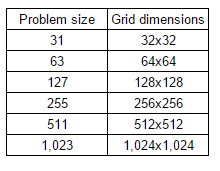
\includegraphics{img/padding}}
\caption[Problem size growth and its effect on the global work size.]{Problem size growth and its effect on the global work size, which denotes the number of work-items to create. The middle column, the total grid size, refers to the size of the actual grid of computational points in the shallow water simulation, including padding.}
\label{t:problemsize}
\end{center}
\end{table}

\section{Results of previous versions}

The previous serial versions (Fortran and C) have been successfully run in the proposed architectures. The compilers used are GCC in the mcore48 (because it is the only C/C++ compiler available for this machine) and Intel icc in the axleman (to link directly with Intel-produced OpenCL libraries on Intel devices). The timing results for the C version obtained in both the mcore48 and the axleman (for CPUs) are in Figure~\ref{f:serial}.

% TODO

\begin{figure}[!h]
\begin{center}
\centerline{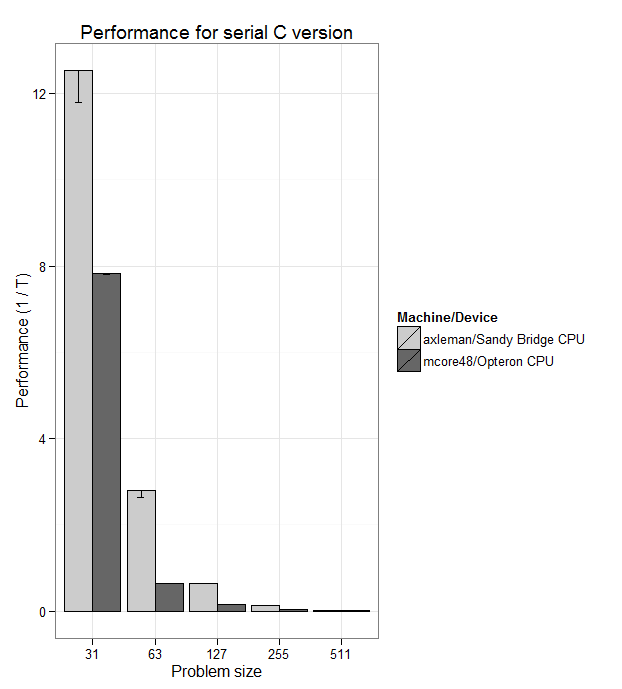
\includegraphics[width=4in]{img/serial}}
\caption{Performance results for serial C version.}
\label{f:serial}
\end{center}
\end{figure}

It can be observed that the Sandy Bridge CPU is faster than the Opteron CPU when using only one core. It may also be noted that performance drops in a non-linear manner when increasing the problem size. While duplicating the problem size means quadrupling the amount of operations that the algorithm will perform,

there are more factors to consider when analysing the scalability of performance on CPUs. Specifically, performance may drop because of the particular characteristics of the hardware used to execute the program.

For instance, one possible cause for additional performance drops in this experiment is the utilisation of slower types of memory (higher levels of cache or RAM) for storing the data of the larger problem. With very small problem sizes, all of the data may fit in the lower, faster levels of cache of a particular CPU used. As the problem size increases, more space is needed for stored data during execution, which may cause cache misses and reduce the performance.

A more comprehensive analysis of the problem sizes, the data needed for the execution of the shallow water simulation, and their relationship with memory types and performance is done in~\cite{pappas2012}. Particular attention is given to the behaviour of performance in multi-core architectures, where other issues like cache coherence and data sharing affect the resulting performance of the algorithm.

\subsection{Results of modifying the local work size}

This section presents the initial experiment of running the code using different configurations of work-group sizes, as shown in~\cite{dolbeau2013one}. The result of this experiment explores the idea that different performance results will be obtained from different work-group sizes, but additional statistical analysis is needed to determine if there is one optimum work-group size that minimises performance losses for all architectures~\cite{dolbeau2013one}.

Work has been directed into understanding the performance of this code when run on the Xeon Phi accelerator to determine whether or not it may be improved upon. The first step was to remove a conditional statement that exists in some of the kernels. As remarked in~\cite{7_software.intel.com_2014}, this branching can prevent the proper vectorisation of the kernels, which is of vital importance to obtaining performance from the Xeon Phi.

As mentioned in the same article, repeatedly calling kernels results in poor performance results when using the Xeon Phi because threads are created with every kernel call. The main loop in the current code calls three different kernels in every iteration. Whether or not this behaviour results in poor performance remains to be proved in this project.

% TODO For the dissertation, a more detailed analysis will be performed using Intel VTune profiler~\cite{7_software.intel.com_2013}.

The OpenCL version has been successfully run in axleman using Sandy Bridge CPU, Tesla GPU and Xeon Phi as different devices, with the same local work sizes as discussed in Chapter 3. The results for the Xeon Phi are in Figure~\ref{f:phi}.

\begin{figure}[!h]
\begin{center}
\centerline{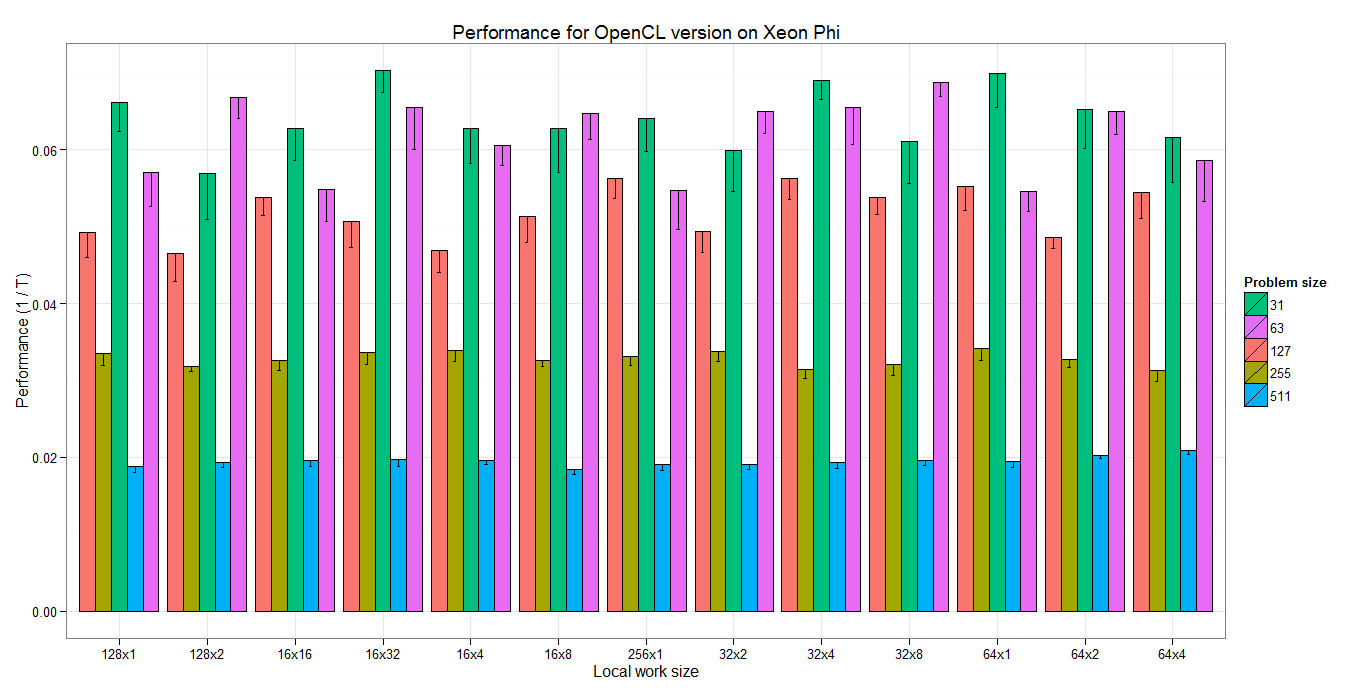
\includegraphics[width=6in]{img/phi}}
\caption{Performance results for OpenCL version running on Xeon Phi.}
\label{f:phi}
\end{center}
\end{figure}

The plot shows that there exist some variations in the performance when tuning the local work size.


\section{OpenCL work partitioning}


\section{CPUs}

When targeting an Intel CPU architecture, the OpenCL device will be a multi-core CPU, or a cluster of multiple CPUs in a multi-socket machine (like the mcore48 or axleman) and each core of the CPU configuration will be an compute unit~\cite{Intel2014}. This means that when a kernel is executed by OpenCL, each work group will be a thread executing on a core~\cite{Sych2014}.



\section{Nvidia GPUs}



\section{Xeon Phi}





\section{}

The local work group sizes used for experimentation have been selected to get better performance results. In the case of CPU-based architectures (the Sandy Bridge CPU and the Xeon Phi), the work group dimensions are chosen so that the allocate



Since the OpenCL version 





\section{}







\section{Summary}

% TODO The current progress of the project has been presented in this chapter. While some interesting observations can be made with the current timing and performance measures, more experiments are needed in order to complete the evaluation of the project, which are planned to be performed in the next tasks of the plan and will be included in the dissertation.
